\chapter{The Search for the Non-resonant Production of Higgs Boson Pairs}
\label{chap:search_hh}

%It was miraculous. It was almost no trick at all, he saw, to turn vice into
%virtue and slander into truth, impotence into abstinence, arrogance into humility,
%plunder into philanthropy, thievery into honor, blasphemy into wisdom, brutality
%into patriotism, and sadism into justice. Anybody could do it; it required no
%brains at all. It merely required no character.

\epigraph{
\textit{It was miraculous... Anybody could do it; it required no brains at all.
It merely required no character.}
}
{
--Joseph Heller, \textit{Catch-22}
}

%\epigraph{
%\textit{Because no battle is ever won he said. They are not even fought. The field only
%reveals to man his own folly and despair, and victory is an illusion of philosophers and fools.}
%}
%{
%--William Faulkner, \textit{The Sound and the Fury}
%}

\epigraph{
\textit{...the ass will carry his load, but not a double load; ride not a free horse to death.}
}
{
--Miguel de Cervantes, \textit{Don Quixote}
}

%%%%%%%%%%%%%%%%%%%%%%%%%%%%%%%%%%%%%%%%%%%%%%%%%%%%%%%%%%%%%%%%%%%%%%%%%%%%%%%%%%%%%
%%%%%%%%%%%%%%%%%%%%%%%%%%%%%%%%%%%%%%%%%%%%%%%%%%%%%%%%%%%%%%%%%%%%%%%%%%%%%%%%%%%%%
%%%%%%%%%%%%%%%%%%%%%%%%%%%%%%%%%%%%%%%%%%%%%%%%%%%%%%%%%%%%%%%%%%%%%%%%%%%%%%%%%%%%%
%
% INTRO
%
%%%%%%%%%%%%%%%%%%%%%%%%%%%%%%%%%%%%%%%%%%%%%%%%%%%%%%%%%%%%%%%%%%%%%%%%%%%%%%%%%%%%%
%%%%%%%%%%%%%%%%%%%%%%%%%%%%%%%%%%%%%%%%%%%%%%%%%%%%%%%%%%%%%%%%%%%%%%%%%%%%%%%%%%%%%
%%%%%%%%%%%%%%%%%%%%%%%%%%%%%%%%%%%%%%%%%%%%%%%%%%%%%%%%%%%%%%%%%%%%%%%%%%%%%%%%%%%%%

In this chapter, the search for the non-resonant production of Higgs boson pairs ($hh$) will be discussed.
As described in {\color{red}{Section XXX}}, the SM predicts non-resonant $hh$ production but with
an exceedingly small overall cross-section of $31.05$\,fb that is $\mathcal{O}(1000)$ times smaller
than that of the dominant production modes of single Higgs bosons:
\begin{align}
    \frac{\sigma_h}{\sigma_{hh}} = \frac{ 4.852 \times 10^3\,\mathrm{fb}}{31.05\,\mathrm{fb}} = 1.56 \times 10^3
    \label{eq:hh_xsec_frac}
\end{align}
The need to complete our understanding of the 125\,GeV Higgs boson, discovered in 2012, requires
that meanginful samples of events containing Higgs pairs are obtained, as the study of these $hh$
events are the only way to have direct measurement of and ability to constrain the Higgs self-coupling parameter $\lambda$
responsible for the structure of the SM vacuum and the onset of EWSB.
At the time of writing, at the end of LHC Run 2, the current $pp$ collision datasets available to the
general purpose LHC experiments are not large enough to observe the $hh$ process as predicted in the SM,
as made obvious by the relation in  Equation~\ref{eq:hh_xsec_frac}.
With 139\,fb$^{-1}$ of data collected during Run 2 of the LHC by the ATLAS detector,
only $\mathcal{O}(1000)$ $hh$ events will have occurred (using the SM-predicted cross-section).
Taking into account the non-100\% acceptance of the detector, the dominant branching fractions
of the Higgs decays, and the experimentally viable channels for $hh$ decays to be observed,
there is no possibility to observe a clearly distinguished $hh$ signal.
With this said, however, there are clear motivations for developing a robust $hh$ search program with the
current $pp$ collision data.
The first being that, given such a small predicted cross-section, \textit{any} observed signal consistent
with $hh$ production in the present data will be an unambiguous sign of new physics.
The second motivation lies in the fact that, considering the LHC timeline (c.f. Figure~\ref{fig:lhc_schedule}), the
forecasted amount of data required to have a $5\sigma$ evidence of $hh$ production, as predicted by the SM,
may yet be out of reach even at the end of the HL-LHC era.

\begin{figure}[!htb]
    \begin{center}
        \includegraphics[width=0.6\textwidth]{figures/search_hh/feynman_diagrams/fdiagram_triangle}
        \includegraphics[width=0.6\textwidth]{figures/search_hh/feynman_diagrams/fdiagram_box}
        \caption{
        }
        \label{fig:hh_feynman}
    \end{center}
\end{figure}

%%%%%%%%%%%%%%%%%%%%%%%%%%%%%%%%%%%%%%%%%%%%%%%%%%%%%%%%%%%%%%%%%%%%%%%%%%%%%%%%%%%%%
%%%%%%%%%%%%%%%%%%%%%%%%%%%%%%%%%%%%%%%%%%%%%%%%%%%%%%%%%%%%%%%%%%%%%%%%%%%%%%%%%%%%%
%%%%%%%%%%%%%%%%%%%%%%%%%%%%%%%%%%%%%%%%%%%%%%%%%%%%%%%%%%%%%%%%%%%%%%%%%%%%%%%%%%%%%
%
% HH PHENO
%
%%%%%%%%%%%%%%%%%%%%%%%%%%%%%%%%%%%%%%%%%%%%%%%%%%%%%%%%%%%%%%%%%%%%%%%%%%%%%%%%%%%%%
%%%%%%%%%%%%%%%%%%%%%%%%%%%%%%%%%%%%%%%%%%%%%%%%%%%%%%%%%%%%%%%%%%%%%%%%%%%%%%%%%%%%%
%%%%%%%%%%%%%%%%%%%%%%%%%%%%%%%%%%%%%%%%%%%%%%%%%%%%%%%%%%%%%%%%%%%%%%%%%%%%%%%%%%%%%

\section{Phenomenology of the Signal}
\label{sec:stop_pheno}

\section{Event Selection and Object Definition}
\label{sec:event_sel}

\section{Signal Selection Strategy}
\label{sec:hh_strategy}

%%%%%%%%%%%%%%%%%%%%%%%%%%%%%%%%%%%%%%%%%%%%%%%%%%%%%%%%%%%%%%%%%%%%%%%%%%%%%%%%%%%
%%%%%%%%%%%%%%%%%%%%%%%%%%%%%%%%%%%%%%%%%%%%%%%%%%%%%%%%%%%%%%%%%%%%%%%%%%%%%%%%%%%
%%%%%%%%%%%%%%%%%%%%%%%%%%%%%%%%%%%%%%%%%%%%%%%%%%%%%%%%%%%%%%%%%%%%%%%%%%%%%%%%%%%
%
% NN 
%
%%%%%%%%%%%%%%%%%%%%%%%%%%%%%%%%%%%%%%%%%%%%%%%%%%%%%%%%%%%%%%%%%%%%%%%%%%%%%%%%%%%
%%%%%%%%%%%%%%%%%%%%%%%%%%%%%%%%%%%%%%%%%%%%%%%%%%%%%%%%%%%%%%%%%%%%%%%%%%%%%%%%%%%
%%%%%%%%%%%%%%%%%%%%%%%%%%%%%%%%%%%%%%%%%%%%%%%%%%%%%%%%%%%%%%%%%%%%%%%%%%%%%%%%%%%


The current analysis makes use of a multi-output classifier, one that does not simply classifry
a single process against a single background label, but rather a classifier that provides multiple
output labels with each pertaining to a distinct class or process.
One of the easiest ways to build such a classifier is to take a multi-variate approach that
is by default suitable for multi-output classification: neural networks.

\subsection{Neural Network Architecture}
\label{sec:nn_arch}

The analysis makes use of a deep-learning, neural network based approach.
The classifiers that we build are trained to classify $pp$ collision events according to
four potential class labels, inspired by the dominant expected background processes:
\begin{enumerate}
    \item Dilepton non-resonant $hh \rightarrow \bbww$
    \item SM top-quark processes ($\ttbar + Wt$), `Top'
    \item SM $Z$+jets processes, $Z \rightarrow \{ee,\mu\mu\}$
    \item SM $Z$+jets processes, $Z \rightarrow \tau\tau$
\end{enumerate}
The classifier is trained with separate labels for the $Z \rightarrow \{ee,\mu\mu\}$ and
$Z \rightarrow \tau\tau$ processes as these lead to clearly different final state kinematics.
The dilepton final state that we eventually select in the analysis is composed only of electrons and muons.
The $Z \rightarrow \tau\tau$ process contributes only in the cases where both $\tau$ leptons decay
leptonically.
The electrons and muons from these $\tau$ decays have very different kinematic signatures as compared
to those from the direct decays of the $Z$-bosons.
Allowing the classifier to learn to distinguish between these $Z$ decays improves its overall performance
to separate the $hh$ signal process from the backgrounds.

%The dominant SM top-quark backgrounds, \ttbar~and single-top $Wt$ are combined into a single
%process during the training of the classifier since these two top-quark processes are found
%to have similar enough kinematics in the regions of high signal purity that separating them
%at the point of training has little effect.
%Additionally, in regions where there is large contributions from both SM \ttbar~and single-top $Wt$
%processes, particularly in the $WWbb$ final state, the two processes have non-trivial quantum
%interferene and it becomes difficult to define them separately.
%For this reason, we consider the sum of these two processes as a single background.

We construct the neural network architecture using the \textsc{Keras}~\cite{chollet2015keras}
library, using \textsc{Tensorflow}~\cite{tensorflow2015} as a backend.
An illustration of the neural network architecture is given in Figure~\ref{fig:nn_arch}.
The network inputs are passed through a dense (fully-connected) layer,  which
is trained with a dropout layer, and then a second dense layer.
The final activation is a softmax activation.

\begin{figure}[!htb]
    \begin{center}
        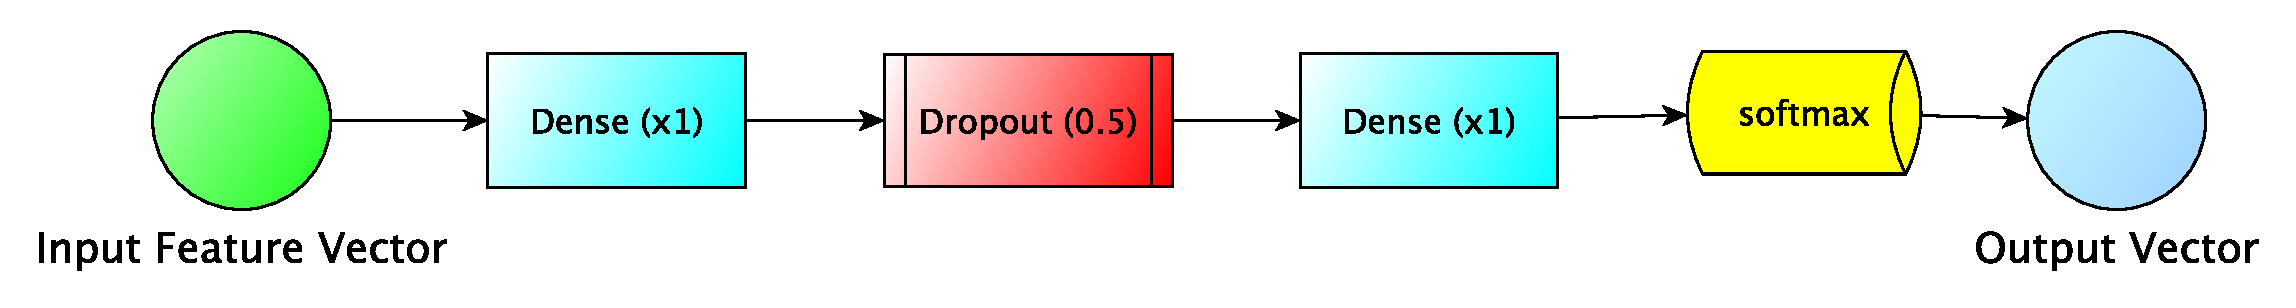
\includegraphics[width=0.85\textwidth]{figures/search_hh/mva/nn_arch_graph_updated}
        \caption{
            Illustration of the neural network graph employed in the analysis.
            The input feature vector has a length of 35 and the output vector is length 4,
            one for each of the targetted processes.
        }
        \label{fig:nn_arch}
    \end{center}
\end{figure}
Each of the dense layers are 250 nodes wide and  have their weights randomly initialized by sampling
from a truncated normal distribution centered on zero with a width given by $\sqrt{1/N_{\text{inputs}}}$, where
$N_{\text{inputs}}$ is the number of input features (the length of the input vector).
The activation functions for each of the dense layers are rectified linear units (`ReLu')~\cite{ReLu}.

Using an output layer with a softmax activation function allows one to interpret the outputs as
each representing a probability\footnote{The use of the term `probability' here is only
loosely correct, as the outputs are not \textit{strictly} probabilities.}
for the output's associated class ($hh$, Top, $Z \rightarrow \{ee,\mu\mu\}$,
or $Z \rightarrow \tau\tau$) given the inputs and for this reason it is commonly used for multi-class
neural network classifiers.
The association of the softmax activation with a class probability can be seen by its definition,
\begin{align}
    a_j = \frac{ e^{z_j} } { \sum\limits_k e ^{z_k} },
    \label{eq:softmax_activation}
\end{align}
where $a_j$ is the activation of the $j^{th}$ output neuron, the $z_i$ are the inputs to the output layer,
and $k$ runs over all output neurons.
It can be seen that if one sums over all outputs of a layer whose activation is given by Equation~\ref{eq:softmax_activation}
that the sum is equal to one.
Thus, the outputs of the softmax layer can be seen as a probability distribution.
For this reason, in the discussion to follow, we refer to the outputs of our neural network as `$p_i$',
where $i$ has four possibiities for each of the four outputs: $i \in \{ hh, \text{Top}, Z\rightarrow ee/\mu\mu, Z\rightarrow \tau\tau \}$.

The use of droput layers during the training process of is a form of statistical learning regularization that is reminiscient
of ensemble methods in the non-deep-learning arena, such as random forests~\cite{RandomForestsBreiman2001}.
They act to randomly disable a tunable fraction of inputs during various points in the training stage~\cite{JMLRDropout}.
This tunable fraction is referred to as the \textit{dropout rate}.
The use of dropout regularization prevents nodes within the network from co-adapting too much, thus reducing
the effects of overtraining.
This is illustrated in Figure~\ref{fig:dropout_illustration}.
During each batch of events forwarded to the network during the training phase, the dropout layer disables
portions of the network and thereby presents a modified network to the inputs.
Conceptually, then, using dropout during training is similar to training a set of very many, different \textit{weak}
neural networks.
During test time, at the time when the neural network is actually being used in the analysis,
the network's weights, which have been determined after training over the set of thinned networks,
are scaled down by the dropout rate.
This is illustrated in Figure~\ref{fig:dropout_weight_scaling}.

\begin{figure}[!htb]
    \begin{center}
        \includegraphics[width=0.85\textwidth]{figures/search_hh/mva/dropout_illustration}
        \caption{
            Illustration of dropout regularization. Figure taken from Ref.~\cite{JMLRDropout}.
            \textit{\textbf{Left}}: A standard neural network with two fully-connected layers.
            \textit{\textbf{Right}}: An example of a thinned network produced by applying dropout to the
                network on the left.
                The units with `X' have been dropped.
        }
        \label{fig:dropout_illustration}
    \end{center}
\end{figure}

\begin{figure}[!htb]
    \begin{center}
        \includegraphics[width=0.85\textwidth]{figures/search_hh/mva/dropout_weight_scaling}
        \caption{
            Illustration of the dropout rate effect on the network weights. Figure taken from Ref.~\cite{JMLRDropout}.
            \textit{\textbf{Left}}: A node in a fully-connected layer at training time is present in the network with
                a probability equal to the dropout rate and is connected to the next layer with weights represented by $\bm{w}$.
            \textit{\textbf{Right}}: At test time, the node is present with 100\% probability but its weights are scaled down by the
                dropout rate, $p\bm{w}$.
        }
        \label{fig:dropout_weight_scaling}
    \end{center}
\end{figure}

\noindent
As mentioned above, the use of dropout regularization prevents nodes within the network from co-adapting
too much and forces the network to learn more robust features that are useful in conjunction with many 
different random subsets of the other nodes.
That is, dropout regularization ensures that the model is robust against the loss of any individual
``piece of evidence'' and is found to reduce the effects of overtraining, which improves the generalizability
of the trained classifier.

The neural network classifier used in the present analysis, illustrated in Figure~\ref{fig:nn_arch},
uses a single dropout layer acting on the first fully-connected node and is given a dropout rate of 50\%.

During training, the loss metric is the categorical crossentropy and the Adam optimization algorithm~\cite{AdamOptimizer} is used.\footnote{More
on categorical cross-entropy: \href{https://ml-cheatsheet.readthedocs.io/en/latest/loss_functions.html\#cross-entropy}
{https://ml-cheatsheet.readthedocs.io/en/latest/loss\_functions.html\#cross-entropy}}


%%%%%%%%%%%%%%%%%%%%%%%%%%%%%%%%%%%%%%%%%%%%%%%%%%%%%%%%%%%%%%%%%%%%%%%%%%%%%%%%%%%
%%%%%%%%%%%%%%%%%%%%%%%%%%%%%%%%%%%%%%%%%%%%%%%%%%%%%%%%%%%%%%%%%%%%%%%%%%%%%%%%%%%
%%%%%%%%%%%%%%%%%%%%%%%%%%%%%%%%%%%%%%%%%%%%%%%%%%%%%%%%%%%%%%%%%%%%%%%%%%%%%%%%%%%
%
% TRAINING AND ARCHITECTURE
%
%%%%%%%%%%%%%%%%%%%%%%%%%%%%%%%%%%%%%%%%%%%%%%%%%%%%%%%%%%%%%%%%%%%%%%%%%%%%%%%%%%%
%%%%%%%%%%%%%%%%%%%%%%%%%%%%%%%%%%%%%%%%%%%%%%%%%%%%%%%%%%%%%%%%%%%%%%%%%%%%%%%%%%%
%%%%%%%%%%%%%%%%%%%%%%%%%%%%%%%%%%%%%%%%%%%%%%%%%%%%%%%%%%%%%%%%%%%%%%%%%%%%%%%%%%%

\section{Estimation of Backgrounds}
\label{sec:stop_background_estimate}

In this section, we describe the methods used for the estimation of the SM background
contamination in the SRs.
By Table~\ref{tab:stop_exp_sr_yield}, it can be seen that the expected SM background
contamination to the SRs in the \bWN search is primarily composed of events
from the \ttbar~and diboson processes.
Given that these are the dominant backgrounds for the analysis, their estimation is performed
using the control region method, described in Section~\ref{sec:control_region_method}.
That is, dedicated CRs and VRs are defined for each of the two processes in order
to provide a normalisation correction for their MC prediction in the SRs.
All other background processes, being subdominant, have their predicted contribution
to the SR background taken directly from the MC simulation.
The estimation of the contribution of sources leading to fake and non-prompt leptons
is performed using the Matrix Method, described in Section~\ref{sec:matrix_method}.

Sections~\ref{sec:stop_ttbar_estimate} and \ref{sec:stop_vv_estimate} describe
the background estimate for the \ttbar~and diboson processes, respectively.

%sub-dominant and FNP via MC alone (shape and normalisation prediction)
%dominant, ttbar and vv, are estimated in a semi-data driven fashion using
% dedicated control regions
%  --> yields tables in CR
%  --> SR normalisation correction factors

The CR and VR definitions for both the \ttbar~and diboson background are based on the
SR definitions given in the previous section.
The CRs are defined primarily by inverting the two-dimensional selection
made in the $(\cosb, \dpb)$-plane, and maintaining similar selections as in the SRs for the other variables.
The VRs, on the other hand, are defined by inverting the selections on the non-angular variables relative to those
made in the SRs.

\begin{figure}[!htb]
    \begin{center}
        \includegraphics[width=0.7\textwidth]{figures/search_stop2l/bkg_est/crvrmotivation}
        \caption{
            Illustration of the CR and VR strategy used in the \bWN search.
            The defining characteristic for the definition of these regions is
            based on the region in the $(\cosb, \dpb)$-plane that they select.
            The CR inverts the requirements on these quantities relative to the SRs,
            while the VR has the same requirements as in the SRs but inverts
            selections made on the other observables.
        }
        \label{fig:stop_crvr_motivation}
    \end{center}
\end{figure}

\FloatBarrier
%%%%%%%%%%%%%%%%%%%%%%%%%%%%%%%%%%%%%%%%%%%%%%%%%%%%%%%%%%%%%%%%%%%%%%%%%%%%%%%%%%%%%%%%%%%%
%%%%%%%%%%%%%%%%%%%%%%%%%%%%%%%%%%%%%%%%%%%%%%%%%%%%%%%%%%%%%%%%%%%%%%%%%%%%%%%%%%%%%%%%%%%%
%%%%%%%%%%%%%%%%%%%%%%%%%%%%%%%%%%%%%%%%%%%%%%%%%%%%%%%%%%%%%%%%%%%%%%%%%%%%%%%%%%%%%%%%%%%%
%
% TOP BKG
%
%%%%%%%%%%%%%%%%%%%%%%%%%%%%%%%%%%%%%%%%%%%%%%%%%%%%%%%%%%%%%%%%%%%%%%%%%%%%%%%%%%%%%%%%%%%%
%%%%%%%%%%%%%%%%%%%%%%%%%%%%%%%%%%%%%%%%%%%%%%%%%%%%%%%%%%%%%%%%%%%%%%%%%%%%%%%%%%%%%%%%%%%%
%%%%%%%%%%%%%%%%%%%%%%%%%%%%%%%%%%%%%%%%%%%%%%%%%%%%%%%%%%%%%%%%%%%%%%%%%%%%%%%%%%%%%%%%%%%%

\subsection{Top-quark pair production}
\label{sec:stop_ttbar_estimate}

The CRs and VRs designed to derive and validate the semi-data-driven
normalisation correction factor for the \ttbar~background process are called
CR-Top and VR-Top, respectively, and are defined in Table~\ref{tab:stop_top_crvr}.
The strategy for the CR and VR selections in the $(\cosb, \dpb)$ plane are described
in the previous section.
Several of the selections on the kinematic quantities relative to those in the SRs (c.f. Table~\ref{tab:stop_sr_def})
are relaxed.
In both CR-Top and VR-Top, the \mdr requirement is relaxed to $\mdr > 80$\,GeV and the requirement on the
\gaminv quantity is removed.
In VR-Top, the \rpt requirement is inverted relative to that used in the SRs.
Given that the \ttbar~background is flavor symmetric, only different-flavor events
are allowed to populate CR-Top and VR-Top, in order to avoid contamination from $Z$-boson processes.
As a result, no additioanl requirement on $m_{\ell\ell}$ is made in these regions.
For increased purity, CR-Top requires that there be at least one $b$-tagged jet,
while VR-Top applies a veto in order to be orthogonal to CR-Top.

VR-Top is defined to have zero $b$-tagged jets, while CR-Top requires at least one.
In dedicated studies, it has been verified that the \ttbar~normalisation correction derived
in the $b$-jet rich region CR-Top is well extrapolated to separate validation regions, and is rather
independent of the $b$-tagged jet multiplicity.
This gives confidence that VR-Top can be used as an appropriate check on the \ttbar~normalisation
correct factor and that it's extrapolation to the SRs, which have differing requirements on the
$b$-tagged jet multiplicity, is reasonable.

Distributions of several key observables in CR-Top are shown in Figures~\ref{fig:crt_0}-\ref{fig:crt_1}.
{\color{red}{VR-TOP DISTRIBUTIONS IN APPENDIX??}}

\begin{table}[!htb]
    \begin{center}
        \begin{scriptsize}
        \caption{
            Definitions of the CR and VR for the \ttbar~background process for the
            \bWN search.
        }
        \label{tab:stop_top_crvr}
        \begin{tabular}{l | c c}
            \hline
            \hline
                & \multicolumn{2}{c}{\textbf{Regions}} \\
            \hline
            \textbf{Variable} & \textbf{CR-Top} & \textbf{VR-Top} \\
            \hline
            Dilepton Flavor & DF & DF \\
            $m_{\ell\ell}$ [GeV]    & no req. & no req. \\
            Lead lepton \pT~[GeV] & $>25$ & $>25$ \\
            Sub-lead lepton \pT~[GeV] & $>20$ & $>20$ \\
            $b$-tagged jet multiplicity & $>0$ & Exactly 0 \\
            \mdr [GeV] & $>80$ & $>80$ \\
            \rpt & $>0.7$ & $<0.7$ \\
            \gaminv & no req. & no req. \\
            $(\cosb, \dpb)$ & \multicolumn{1}{c}{\small{$\dpb < 0.9 \times | \cosb | + 1.6$}} & \multicolumn{1}{c}{\small{$\dpb> 0.9 \times | \cosb | + 1.6$}} \\
            %$(\cosb, \dpb)$ & $\dpb $ & $\dpb$ \\
            %        & \hspace{1.8cm} $< 0.9 \times | \cosb | + 1.6$ & \hspace{1.8cm}$> 0.9 \times | \cosb | + 1.6$ \\
            \hline
            \hline
        \end{tabular}
        \end{scriptsize}
    \end{center}
\end{table}

\subsubsection{Kinematic Distributions in CR-Top}

\begin{figure}[!htb]
    \begin{center}
        \includegraphics[width=0.48\textwidth]{figures/search_stop2l/bkg_est/crtop/crt_MDR}
        \includegraphics[width=0.48\textwidth]{figures/search_stop2l/bkg_est/crtop/crt_l_pt0}
        \includegraphics[width=0.48\textwidth]{figures/search_stop2l/bkg_est/crtop/crt_DPB_vSS}
        \includegraphics[width=0.48\textwidth]{figures/search_stop2l/bkg_est/crtop/crt_cosThetaB}
        \caption{
            Distributions of \mdr (\textit{upper left}), leading lepton \pT~(\textit{upper right}),
            \dpb (\textit{lower left}), and $|\cosb|$ (\textit{lower right}) in the \ttbar CR,
            CR-Top.
            The error on the SM processes includes statistical and systematic uncertainties.
            The post-fit normalization correction factors for the \ttbar and diboson processes
            have been applied.
        }
        \label{fig:crt_0}
    \end{center}
\end{figure}
\begin{figure}[!htb]
    \begin{center}
        \includegraphics[width=0.48\textwidth]{figures/search_stop2l/bkg_est/crtop/crt_RPT}
        \includegraphics[width=0.48\textwidth]{figures/search_stop2l/bkg_est/crtop/crt_gamInvRp1}
        \includegraphics[width=0.48\textwidth]{figures/search_stop2l/bkg_est/crtop/crt_nBJets}
        \includegraphics[width=0.48\textwidth]{figures/search_stop2l/bkg_est/crtop/crt_nSJets}
        \caption{
            Distributions of \rpt (\textit{upper left}), leading lepton \gaminv~(\textit{upper right}),
            $b$-tagged jet multiplicity (\textit{lower left}), and non-$b$-tagged jet multiplicity(\textit{lower right}) in the \ttbar CR,
            CR-Top.
            The error on the SM processes includes statistical and systematic uncertainties.
            The post-fit normalization correction factors for the \ttbar and diboson processes
            have been applied.
        }
        \label{fig:crt_1}
    \end{center}
\end{figure}



%%%%%%%%%%%%%%%%%%%%%%%%%%%%%%%%%%%%%%%%%%%%%%%%%%%%%%%%%%%%%%%%%%%%%%%%%%%%%%%%%%%%%%%%%%%%
%%%%%%%%%%%%%%%%%%%%%%%%%%%%%%%%%%%%%%%%%%%%%%%%%%%%%%%%%%%%%%%%%%%%%%%%%%%%%%%%%%%%%%%%%%%%
%%%%%%%%%%%%%%%%%%%%%%%%%%%%%%%%%%%%%%%%%%%%%%%%%%%%%%%%%%%%%%%%%%%%%%%%%%%%%%%%%%%%%%%%%%%%
%
% VV BKG
%
%%%%%%%%%%%%%%%%%%%%%%%%%%%%%%%%%%%%%%%%%%%%%%%%%%%%%%%%%%%%%%%%%%%%%%%%%%%%%%%%%%%%%%%%%%%%
%%%%%%%%%%%%%%%%%%%%%%%%%%%%%%%%%%%%%%%%%%%%%%%%%%%%%%%%%%%%%%%%%%%%%%%%%%%%%%%%%%%%%%%%%%%%
%%%%%%%%%%%%%%%%%%%%%%%%%%%%%%%%%%%%%%%%%%%%%%%%%%%%%%%%%%%%%%%%%%%%%%%%%%%%%%%%%%%%%%%%%%%%

\subsection{Diboson Production}
\label{sec:stop_vv_estimate}

The SM diboson processes are composed of $WW$, $ZW+WZ$, and $ZZ$ production.
The dominant process for the \bWN SRs is $WW$, as discussed in the text.
In order to constrain the $WW$ component, in addition to those components with a $Z$ boson,
the diboson CRs are split into two, one targetting the different-flavor enriched component
of the diboson background (predominantly $WW$) and one in which the same-flavor component ($ZW+WZ$ and $ZZ$)
is enriched.

The same-flavor and different-flavor diboson CRs (VRs), CR-VV-SF and CR-VV-DF (VR-VV-SF and VR-VV-DF), respectively,
are defined in Table~\ref{tab:stop_vv_crvr}.
All of the regions apply a $b$-tagged jet veto.
Although there are SRs that are inclusive of $b$-tagged jets (SRt-SF and SRt-DF), the diboson background
is negligible in them and so the normalisation correction factors derived in the diboson CRs
can be extrapolated with confidence into the SRs with a $b$-tagged jet veto (SRw-SF and SRw-DF).
There is no difference between the same-flavor and different-flavor CRs, apart from the dilepton flavor
requirements and $Z$-veto.
The diboson VRs have the same, or inclusive, \rpt and \gaminv  selections as the CRs but have orthogonal
\mdr requirements that move them closer the SR selections.

Distributions of several key observables in CR-VV-SF (CR-VV-DF) are shown in Figures~\ref{fig:crvvSF_0}-\ref{fig:crvvSF_1}
(Figures~\ref{fig:crvvDF_0}-\ref{fig:crvvDF_1}).

{\color{red}{VR-VV DISTRIBUTIONS IN APPENDIX??}}

\begin{table}[!htb]
    \begin{center}
        \begin{scriptsize}
        \caption{
            Definitions of the CR and VR for the diboson~background processes for the
            \bWN search.
        }
        \label{tab:stop_vv_crvr}
        \begin{tabular}{l | c c c c}
            \hline
            \hline
                & \multicolumn{4}{c}{\textbf{Regions}} \\
            \hline
            \textbf{Variable} & \textbf{CR-VV-DF} & \textbf{CR-VV-SF} & \textbf{VR-VV-DF} & \textbf{VR-VV-SF} \\
            \hline
            Dilepton Flavor & DF & SF & DF & SF \\
            $m_{\ell\ell}$ [GeV]    & no req. & $|m_{\ell\ell} - 91.2| > 10$ & no req. & $|m_{\ell\ell} - 91.2| > 10$ \\
            Lead lepton \pT~[GeV] & $>25$ & $>25$ & $>25$ & $>25$ \\
            Sub-lead lepton \pT~[GeV] & $>20$ & $>20$ & $>20$ & $>20$ \\
            $b$-tagged jet multiplicity & Exactly 0 & Exactly 0 & Exactly 0 & Exactly 0 \\
            \mdr [GeV] & $>50$ & $>70$ & $\in(50,95)$ & $\in(60,95)$ \\
            \rpt & $<0.5$ & $<0.5$ & $<0.7$ & $<0.4$ \\
            \gaminv &  $>0.7$ & $>0.7$ & $>0.7$ & $>0.7$ \\
            $(\cosb, \dpb)$ & \multicolumn{2}{c}{\small{$\dpb < 0.9 \times | \cosb | + 1.6$}} & \multicolumn{2}{c}{\small{$\dpb> 0.9 \times | \cosb | + 1.6$}} \\
%            $(\cosb, \dpb)$ & $\dpb $  &  $\dpb$ & \\
%                    & \hspace{1.8cm} $< 0.9 \times | \cosb | + 1.6$  & \hspace{1.8cm}$> 0.9 \times | \cosb | + 1.6$ \\
            \hline
            \hline
        \end{tabular}
        \end{scriptsize}
    \end{center}
\end{table}

\begin{figure}[!htb]
    \begin{center}
        \includegraphics[width=0.48\textwidth]{figures/search_stop2l/bkg_est/crvsf/crvSF_MDR}
        \includegraphics[width=0.48\textwidth]{figures/search_stop2l/bkg_est/crvsf/crvSF_l_pt0}
        \includegraphics[width=0.48\textwidth]{figures/search_stop2l/bkg_est/crvsf/crvSF_DPB_vSS}
        \includegraphics[width=0.48\textwidth]{figures/search_stop2l/bkg_est/crvsf/crvSF_cosThetaB}
        \caption{
            Distributions of \mdr (\textit{upper left}), leading lepton \pT~(\textit{upper right}),
            \dpb (\textit{lower left}), and $|\cosb|$ (\textit{lower right}) in the same-flavor diboson CR,
            CR-VV-SF.
            The error on the SM processes includes statistical and systematic uncertainties.
            The post-fit normalization correction factors for the \ttbar and diboson processes
            have been applied.
        }
        \label{fig:crvvSF_0}
    \end{center}
\end{figure}
\begin{figure}[!htb]
    \begin{center}
        \includegraphics[width=0.48\textwidth]{figures/search_stop2l/bkg_est/crvsf/crvSF_RPT}
        \includegraphics[width=0.48\textwidth]{figures/search_stop2l/bkg_est/crvsf/crvSF_gamInvRp1}
        \includegraphics[width=0.48\textwidth]{figures/search_stop2l/bkg_est/crvsf/crvSF_nBJets}
        \includegraphics[width=0.48\textwidth]{figures/search_stop2l/bkg_est/crvsf/crvSF_nSJets}
        \caption{
            Distributions of \rpt (\textit{upper left}), leading lepton \gaminv~(\textit{upper right}),
            $b$-tagged jet multiplicity (\textit{lower left}), and non-$b$-tagged jet multiplicity(\textit{lower right}) in the same-flavor diboson CR,
            CR-VV-SF.
            The error on the SM processes includes statistical and systematic uncertainties.
            The post-fit normalization correction factors for the \ttbar and diboson processes
            have been applied.
        }
        \label{fig:crvvSF_1}
    \end{center}
\end{figure}

\begin{figure}[!htb]
    \begin{center}
        \includegraphics[width=0.48\textwidth]{figures/search_stop2l/bkg_est/crvdf/crv_MDR}
        \includegraphics[width=0.48\textwidth]{figures/search_stop2l/bkg_est/crvdf/crv_l_pt0}
        \includegraphics[width=0.48\textwidth]{figures/search_stop2l/bkg_est/crvdf/crv_DPB_vSS}
        \includegraphics[width=0.48\textwidth]{figures/search_stop2l/bkg_est/crvdf/crv_cosThetaB}
        \caption{
            Distributions of \mdr (\textit{upper left}), leading lepton \pT~(\textit{upper right}),
            \dpb (\textit{lower left}), and $|\cosb|$ (\textit{lower right}) in the different-flavor diboson CR,
            CR-VV-DF.
            The error on the SM processes includes statistical and systematic uncertainties.
            The post-fit normalization correction factors for the \ttbar and diboson processes
            have been applied.
        }
        \label{fig:crvvDF_0}
    \end{center}
\end{figure}
\begin{figure}[!htb]
    \begin{center}
        \includegraphics[width=0.48\textwidth]{figures/search_stop2l/bkg_est/crvdf/crv_RPT}
        \includegraphics[width=0.48\textwidth]{figures/search_stop2l/bkg_est/crvdf/crv_gamInvRp1}
        \includegraphics[width=0.48\textwidth]{figures/search_stop2l/bkg_est/crvdf/crv_nBJets}
        \includegraphics[width=0.48\textwidth]{figures/search_stop2l/bkg_est/crvdf/crv_nSJets}
        \caption{
            Distributions of \rpt (\textit{upper left}), leading lepton \gaminv~(\textit{upper right}),
            $b$-tagged jet multiplicity (\textit{lower left}), and non-$b$-tagged jet multiplicity(\textit{lower right}) in the different-flavor diboson CR,
            CR-VV-DF.
            The error on the SM processes includes statistical and systematic uncertainties.
            The post-fit normalization correction factors for the \ttbar and diboson processes
            have been applied.
        }
        \label{fig:crvvDF_1}
    \end{center}
\end{figure}

\FloatBarrier
%%%%%%%%%%%%%%%%%%%%%%%%%%%%%%%%%%%%%%%%%%%%%%%%%%%%%%%%%%%%%%%%%%%%%%%%%%%%%%%%%%%%%%%%%%%%
%%%%%%%%%%%%%%%%%%%%%%%%%%%%%%%%%%%%%%%%%%%%%%%%%%%%%%%%%%%%%%%%%%%%%%%%%%%%%%%%%%%%%%%%%%%%
%%%%%%%%%%%%%%%%%%%%%%%%%%%%%%%%%%%%%%%%%%%%%%%%%%%%%%%%%%%%%%%%%%%%%%%%%%%%%%%%%%%%%%%%%%%%
%
% POST FIT
%
%%%%%%%%%%%%%%%%%%%%%%%%%%%%%%%%%%%%%%%%%%%%%%%%%%%%%%%%%%%%%%%%%%%%%%%%%%%%%%%%%%%%%%%%%%%%
%%%%%%%%%%%%%%%%%%%%%%%%%%%%%%%%%%%%%%%%%%%%%%%%%%%%%%%%%%%%%%%%%%%%%%%%%%%%%%%%%%%%%%%%%%%%
%%%%%%%%%%%%%%%%%%%%%%%%%%%%%%%%%%%%%%%%%%%%%%%%%%%%%%%%%%%%%%%%%%%%%%%%%%%%%%%%%%%%%%%%%%%%

\subsection{Background-only Fit}
\label{sec:stop_background_only}

In order to assess the impact of the CRs on the background estimation in the SRs, a so-called `background-only'
fit is performed.
A background-only fit is profile-likelihood fit, as described Section~\ref{sec:likelihood},
in which the only regions contributing to the likelihood (c.f Equation~\ref{eq:full_likelihood})
are the analysis' CRs.
The result of running a background-only fit to data in the CRs is shown in Table~\ref{tab:bkgonly_CRVR},
which shows the MC predicted yields for the background processes both before and after the
background-only fit is performed, as well as the observed data counts, in each of the CRs and VRs in the analysis.
The post-fit yields in the CRs are expected to agree with the observed data counts, since the latter are used
as constraints in the fit model and there are as many freely-floating parameters in the fit (3 $\mu$ factors)
as there are CRs; therefore, the fit has enough freedom to cover any discrepancy between the observed data and pre-fit MC prediction of
the background processes.
The agreement observed between the post-fit MC and the observed data in the VRs shows that the extrapolation,
at least in terms of the corrected MC's normalisation, is performing well.

The normalisation correction factors for the \ttbar~and diboson processes obtained in the background-only
fit are listed in Table~\ref{tab:stop_scalefactors}.
They are generally consistent with one.

\begin{table}[!htb]
\begin{center}
\setlength{\tabcolsep}{0.0pc}
{\scriptsize
\caption{
Yields in the \ttbar~and diboson CRs and VRs for the \bWN search for the main background processes
contributing to the analysis.
The lower-portion of the table are the yields before the background-only fit to data
in the CRs, without the normalisation corrections applied.
The upper-portion of the table are those taken after the background-only fit to data.
The errors on the quoted numbers are due to the statistical and experimental systematic uncertainties.
}
\label{tab:bkgonly_CRVR}
\begin{tabular*}{\textwidth}{@{\extracolsep{\fill}}lrrrrrr}
\noalign{\smallskip}\hline\noalign{\smallskip}
\noalign{\smallskip}\hline\noalign{\smallskip}
\textbf{Process}           & \textbf{CR-Top}            & \textbf{CR-VV-DF}            & \textbf{CR-VV-SF}            & \textbf{VR-Top}           & \textbf{VR-VV-DF}            & \textbf{VR-VV-SF}              \\[-0.05cm]
\noalign{\smallskip}\hline\noalign{\smallskip}


Observed Data         & $951$              & $2046$              & $1275$              & $1197$              & $1896$              & $783$                    \\
\noalign{\smallskip}\hline\noalign{\smallskip}
%%
Post-fit Total SM         & $951.00 \pm 30.84$          & $2046.05 \pm 45.23$          & $1275.17 \pm 35.68$          & $1231.78 \pm 86.59$          & $2013.57 \pm 116.49$          & $780.44 \pm 117.32$              \\
\noalign{\smallskip}\hline\noalign{\smallskip}
%%
        Post-fit \ttbar          & $833.03 \pm 32.85$          & $619.74 \pm 111.40$          & $333.62 \pm 60.91$          & $733.87 \pm 64.91$          & $754.94 \pm 78.17$          & $127.14 \pm 22.09$              \\
%%
        Post-fit Diboson (DF)          & $11.51 \pm 2.43$          & $1093.28 \pm 125.83$          & $0.00 \pm 0.00$          & $331.13 \pm 82.57$          & $886.53 \pm 168.16$          & $0.00 \pm 0.00$              \\
%%
        Post-fit Diboson (SF)          & $0.00 \pm 0.00$          & $0.00 \pm 0.00$          & $378.94 \pm 124.32$          & $0.00 \pm 0.00$          & $0.00 \pm 0.00$          & $380.00 \pm 141.58$              \\
%%
        Post-fit Single-top          & $101.10 \pm 9.73$          & $186.47 \pm 27.99$          & $103.47 \pm 17.43$          & $111.52 \pm 14.49$          & $151.88 \pm 14.37$          & $36.40 \pm 5.62$              \\
%%
        Post-fit $\ttbar+V$          & $4.35 \pm 0.42$          & $0.39 \pm 0.07$          & $0.36 \pm 0.07$          & $1.27 \pm 0.22$          & $0.42 \pm 0.13$          & $0.05 \pm 0.02$              \\
%%
        Post-fit $Z$+jets          & $0.70 \pm 0.22$          & $1.83_{-1.83}^{+2.55}$          & $428.58 \pm 92.55$          & $0.47_{-0.47}^{+0.85}$          & $0.39_{-0.39}^{+0.71}$          & $191.37 \pm 78.38$              \\
%%
        Post-fit Single-higgs          & $0.31 \pm 0.13$          & $78.95 \pm 9.17$          & $6.23 \pm 1.06$          & $0.44_{-0.44}^{+0.52}$          & $54.98 \pm 4.34$          & $9.40 \pm 1.11$              \\
%%
        Post-fit Fakes          & $0.00 \pm 0.00$          & $65.37 \pm 2.22$          & $23.96 \pm 1.25$          & $53.09 \pm 1.92$          & $164.42 \pm 5.68$          & $36.09 \pm 3.04$              \\
%%
 \noalign{\smallskip}\hline\noalign{\smallskip}
%%
 Total SM               & $905.14 \pm 16.54$          & $1988.38 \pm 110.43$          & $1248.21 \pm 123.42$          & $1184.39 \pm 71.23$          & $1952.92 \pm 61.72$          & $764.65 \pm 99.06$              \\
\noalign{\smallskip}\hline\noalign{\smallskip}
%%
         \ttbar          & $787.43 \pm 11.29$          & $585.87 \pm 102.00$          & $315.39 \pm 55.87$          & $693.71 \pm 53.51$          & $713.64 \pm 66.57$          & $120.19 \pm 20.17$              \\
%%
         Diboson (DF)          & $11.25 \pm 1.62$          & $1069.46 \pm 12.45$          & $0.00 \pm 0.00$          & $323.89 \pm 50.27$          & $867.18 \pm 77.75$          & $0.00 \pm 0.00$              \\
%%
         Diboson (SF)          & $0.00 \pm 0.00$          & $0.00 \pm 0.00$          & $370.13 \pm 15.48$          & $0.00 \pm 0.00$          & $0.00 \pm 0.00$          & $371.16 \pm 34.38$              \\
%%
         Single-top          & $101.10 \pm 9.80$          & $186.49 \pm 28.25$          & $103.49 \pm 17.59$          & $111.52 \pm 14.60$          & $151.88 \pm 14.46$          & $36.41 \pm 5.66$              \\
%%
         $\ttbar+V$          & $4.35 \pm 0.42$          & $0.39 \pm 0.07$          & $0.36 \pm 0.07$          & $1.27 \pm 0.23$          & $0.42 \pm 0.13$          & $0.05 \pm 0.02$              \\
%%
         $Z$+jets          & $0.70 \pm 0.23$          & $1.83_{-1.83}^{+2.57}$          & $428.65 \pm 93.15$          & $0.48_{-0.48}^{+0.86}$          & $0.40_{-0.40}^{+0.72}$          & $191.36 \pm 78.78$              \\
%%
         Single-higgs          & $0.31 \pm 0.13$          & $78.96 \pm 9.26$          & $6.23 \pm 1.07$          & $0.44_{-0.44}^{+0.53}$          & $54.98 \pm 4.37$          & $9.40 \pm 1.12$              \\
%%
         Fakes          & $0.00 \pm 0.00$          & $65.37 \pm 2.23$          & $23.96 \pm 1.26$          & $53.09 \pm 1.92$          & $164.42 \pm 5.70$          & $36.09 \pm 3.04$              \\
\noalign{\smallskip}\hline\noalign{\smallskip}
\noalign{\smallskip}\hline\noalign{\smallskip}
\end{tabular*}
}
\end{center}
\end{table}

\begin{table}[!htb]
    \begin{center}
        \caption{
            Normalisation correction factors for the \ttbar~$(\mu_{\ttbar})$,
            same-flavor diboson $(\mu_{\text{VV-SF}})$, and different-flavor diboson $(\mu_{\text{VV-DF}})$
            processes derived from the background-only fit to the CRs.
            The errors on the quoted numbers are due to the statistical and experimental systematic uncertainties
            entering the fit.
        }
        \label{tab:stop_scalefactors}
        \begin{tabular}{l|c}
            \hline
            \hline
                $\mu_{\ttbar}$ & $1.06 \pm 0.05$ \\
                $\mu_{\text{VV-SF}}$ & $1.02 \pm 0.12$ \\
                $\mu_{\text{VV-DF}}$ & $1.02 \pm 0.35$ \\
            \hline
            \hline
        \end{tabular}
    \end{center}
\end{table}


\section{Results}
\label{sec:stop_results}

